% Options for packages loaded elsewhere
\PassOptionsToPackage{unicode}{hyperref}
\PassOptionsToPackage{hyphens}{url}
%
\documentclass[
  ignorenonframetext,
  aspectratio=169,
]{beamer}
\usepackage{pgfpages}
\setbeamertemplate{caption}[numbered]
\setbeamertemplate{caption label separator}{: }
\setbeamertemplate{navigation symbols}{}
\setbeamertemplate{footline}[page number]
\setbeamertemplate{itemize item}{\small\raise0.5pt\hbox{$\bullet$}}
\setbeamertemplate{itemize subitem}{\tiny\raise1.5pt\hbox{$\bullet$}}
\setbeamertemplate{itemize subsubitem}{\tiny\raise1.5pt\hbox{$\bullet$}}
\setbeamercolor{caption name}{fg=normal text.fg}
\beamertemplatenavigationsymbolsempty
% Prevent slide breaks in the middle of a paragraph
\widowpenalties 1 10000
\raggedbottom
\setbeamertemplate{part page}{
  \centering
  \begin{beamercolorbox}[sep=16pt,center]{part title}
    \usebeamerfont{part title}\insertpart\par
  \end{beamercolorbox}
}
\setbeamertemplate{section page}{
  \centering
  \begin{beamercolorbox}[sep=12pt,center]{part title}
    \usebeamerfont{section title}\insertsection\par
  \end{beamercolorbox}
}
\setbeamertemplate{subsection page}{
  \centering
  \begin{beamercolorbox}[sep=8pt,center]{part title}
    \usebeamerfont{subsection title}\insertsubsection\par
  \end{beamercolorbox}
}
\AtBeginPart{
  \frame{\partpage}
}
\AtBeginSection{
  \ifbibliography
  \else
    \frame{\sectionpage}
  \fi
}
\AtBeginSubsection{
  \frame{\subsectionpage}
}
\usepackage{amsmath,amssymb}
\usepackage{lmodern}
\usepackage{iftex}
\ifPDFTeX
  \usepackage[T1]{fontenc}
  \usepackage[utf8]{inputenc}
  \usepackage{textcomp} % provide euro and other symbols
\else % if luatex or xetex
  \ifXeTeX
    \usepackage{xltxtra} 
    \usepackage{xeCJK}
    \setCJKmainfont{ipaexm.ttf}
    \setCJKsansfont{ipaexg.ttf}
    \setCJKmonofont{ipaexg.ttf}
  \fi
  \usepackage{unicode-math}
  \defaultfontfeatures{Scale=MatchLowercase}
  \defaultfontfeatures[\rmfamily]{Ligatures=TeX,Scale=1}
\fi
% Use upquote if available, for straight quotes in verbatim environments
\IfFileExists{upquote.sty}{\usepackage{upquote}}{}
\IfFileExists{microtype.sty}{% use microtype if available
  \usepackage[]{microtype}
  \UseMicrotypeSet[protrusion]{basicmath} % disable protrusion for tt fonts
}{}
\makeatletter
\@ifundefined{KOMAClassName}{% if non-KOMA class
  \IfFileExists{parskip.sty}{%
    \usepackage{parskip}
  }{% else
    \setlength{\parindent}{0pt}
    \setlength{\parskip}{6pt plus 2pt minus 1pt}}
}{% if KOMA class
  \KOMAoptions{parskip=half}}
\makeatother
\usepackage{xcolor}
\IfFileExists{xurl.sty}{\usepackage{xurl}}{} % add URL line breaks if available
\IfFileExists{bookmark.sty}{\usepackage{bookmark}}{\usepackage{hyperref}}
\hypersetup{
  pdftitle={Estimating Effect of Tax Incentives on Charitable Giving Considering Self-Selection of Tax Relief in South Korea},
  hidelinks,
  pdfcreator={LaTeX via pandoc}}
\urlstyle{same} % disable monospaced font for URLs

\usepackage{setspace}
\usepackage{float}

\newif\ifbibliography
\usepackage{longtable,booktabs,array}
\usepackage{threeparttable, threeparttablex, multirow}
\usepackage{calc} % for calculating minipage widths
\usepackage{caption}
% Make caption package work with longtable
\makeatletter
\def\fnum@table{\tablename~\thetable}
\makeatother
\usepackage{graphicx}
\makeatletter
\def\maxwidth{\ifdim\Gin@nat@width>\linewidth\linewidth\else\Gin@nat@width\fi}
\def\maxheight{\ifdim\Gin@nat@height>\textheight\textheight\else\Gin@nat@height\fi}
\makeatother
% Scale images if necessary, so that they will not overflow the page
% margins by default, and it is still possible to overwrite the defaults
% using explicit options in \includegraphics[width, height, ...]{}
\setkeys{Gin}{width=\maxwidth,height=\maxheight,keepaspectratio}
% Set default figure placement to htbp
\makeatletter
\def\fps@figure{htbp}
\makeatother
\setlength{\emergencystretch}{3em} % prevent overfull lines
\providecommand{\tightlist}{%
  \setlength{\itemsep}{0pt}\setlength{\parskip}{0pt}}
\setcounter{secnumdepth}{-\maxdimen} % remove section numbering
\newlength{\cslhangindent}
\setlength{\cslhangindent}{1.5em}
\newlength{\csllabelwidth}
\setlength{\csllabelwidth}{3em}
\newlength{\cslentryspacingunit} % times entry-spacing
\setlength{\cslentryspacingunit}{\parskip}
\newenvironment{CSLReferences}[2] % #1 hanging-ident, #2 entry spacing
 {% don't indent paragraphs
  \setlength{\parindent}{0pt}
  % turn on hanging indent if param 1 is 1
  \ifodd #1
  \let\oldpar\par
  \def\par{\hangindent=\cslhangindent\oldpar}
  \fi
  % set entry spacing
  \setlength{\parskip}{#2\cslentryspacingunit}
 }%
 {}
\usepackage{calc}
\newcommand{\CSLBlock}[1]{#1\hfill\break}
\newcommand{\CSLLeftMargin}[1]{\parbox[t]{\csllabelwidth}{#1}}
\newcommand{\CSLRightInline}[1]{\parbox[t]{\linewidth - \csllabelwidth}{#1}\break}
\newcommand{\CSLIndent}[1]{\hspace{\cslhangindent}#1}


\ifLuaTeX
  \usepackage{selnolig}  % disable illegal ligatures
\fi

\title{Estimating Effect of Tax Incentives on Charitable Giving Considering Self-Selection of Tax Relief in South Korea  }
\author[shortname]{ Hiroki Kato \inst{1} \and  Tsuyoshi Goto \inst{2} \and  Yong-Rok Kim \inst{3} \and }
\institute[shortinst]{ \inst{1} Osaka University \and  \inst{2} Chiba University \and  \inst{3} Kansai University \and }

\date{2021/12/17}


\begin{document}
\frame{\titlepage}

\begin{frame}{Introduction}
\protect\hypertarget{introduction}{}
\begin{itemize}
\tightlist
\item
  In many countries, tax relief for charitable giving are implemented.
\item
  The elasticity of giving tax relief is known as a key parameter to evaluate the welfare implication (Saez, 2004).

  \begin{itemize}
  \tightlist
  \item
    Intuitively, if the elasticity is more than 1 in absolute value, \$1 of tax relief make more than \$1 of charitable giving.
  \end{itemize}
\item
  Many papers investigate the elasticity based on tax return data (Almunia et al., 2020; Auten et al., 2002).
\end{itemize}
\end{frame}

\begin{frame}{Introduction}
\protect\hypertarget{introduction-1}{}
\begin{itemize}
\tightlist
\item
  However, the tax return data record only the declared charitable giving.

  \begin{itemize}
  \tightlist
  \item
    First issue: \textbf{Actual donations is different from declared donations.} (Fack and Landais, 2016; Gillitzer and Skov, 2018)
  \item
    We use panel survey data in South Korea to deal with this issue.
  \end{itemize}
\item
  Tax payers decide the amount of donation and whether to declare tax relief based on the size of tax incentive and declaration cost.

  \begin{itemize}
  \tightlist
  \item
    Second issue: Neglect of this declaration cost may bias the estimations of elasticity.
  \item
    We use instrumental variable (IV) and control function approach for this issue.
  \end{itemize}
\item
  Based on DID as an identification strategy, we investigate the giving price elasticity of South Korea.
\end{itemize}
\end{frame}

\begin{frame}{Introduction}
\protect\hypertarget{introduction-2}{}
Result

\begin{enumerate}
\tightlist
\item
  Baseline results show that the giving price elasticity is less than -1.4 in terms of intensive margins and less than -1.7 in terms of extensive margins in Korea.
\item
  The estimated giving price elasticity for those who declare charitable giving is around -1.2 -1.6.

  \begin{itemize}
  \tightlist
  \item
    These estimates are more elastic than the estimates in the extant research, many of which show around -1.
  \end{itemize}
\item
  By reducing application cost, we can increase charitable giving.
\item
  Given our estimates, increasing the subsidy on charitable giving will be desirable in Korea.
\end{enumerate}
\end{frame}

\hypertarget{conceptual-framework}{%
\section{Conceptual Framework}\label{conceptual-framework}}

\begin{frame}{Optimization Problem}
\protect\hypertarget{optimization-problem}{}
Following Almunia et al. (2020),
consider allocation problem between private consumption (\(x_{it}\)) and charitable giving (\(g_{it}\))

\begin{align}
  \max_{x_{it}, g_{it}, R_{it}} &U(x_{it}, g_{it}, G_t)
  = u_i(x_{it}, g_{it}, G_t) - R_{it}K(Z_{it}), \\
  \text{s.t.}\:\:
  &x_{it} + g_{it}
  = y_{it} - R_{it} T_{it}(y_{it}, g_{it}) - (1 - R_{it}) T_{it}(y_{it}), \\
  &G_t = g_{it} + G_{-it},
\end{align}

where \(y_{it}\) is pre-tax total income, \(R_{it}\) is a dummy of declaration of tax relief and \(T_{it}(y_{it})\) and \(T_{it}(y_{it}, g_{it})\) are respectively the amount of tax when \(i\) does not declare tax relief and when \(i\) declares tax relief in year \(t\). \(G_{-it}\) is public goods supplied by others. \(K(Z_{it})\) is application cost which is a function of instrument \(Z_{it}\).
\end{frame}

\begin{frame}{Remarks on Optimization Problem}
\protect\hypertarget{remarks-on-optimization-problem}{}
We assume

\begin{itemize}
\tightlist
\item
  No saving
\item
  \(G_{-it}\) is large enough to \(\frac{\partial u_i}{\partial G}(x, g, G) \approx 0\)
\end{itemize}

Given \(R_{it}\), optimal level of donations sloves

\begin{align}
  \max_{g_{it}} u_i(
    y_{it} - R_{it} T_{it}(y_{it}, g_{it}) - (1 - R_{it}) T_{it}(y_{it}) - g_{it}, g_{it}, g_{it} + G_{-it}
  ).
\end{align}

\begin{itemize}
\tightlist
\item
  We can ignore application cost \(K(Z_{it})\) when solving optimal giving level because the application cost does not depend on \(g_{it}\)
\end{itemize}
\end{frame}

\begin{frame}{First-Order Condition}
\protect\hypertarget{first-order-condition}{}
\begin{align}
  - \frac{\partial u_i}{\partial x_{it}}
  \left( R_{it} \frac{\partial T_{it}}{\partial g_{it}}(y_{it}, g_{it}) + 1 \right)
  + \frac{\partial u_i}{\partial g_{it}} = 0
\end{align}

\begin{itemize}
\tightlist
\item
  \(\partial T_{it} / \partial g_{it} < 0\) is tax incentive of charitable giving.

  \begin{itemize}
  \tightlist
  \item
    Let \(s_{it} \equiv |\partial T_{it} / \partial g_{it}|\) be size of tax incentive.
  \item
    Relative giving price is \(1 - s_{it}\)
  \item
    As we explain later, there is \emph{within} variation of \(s_{it}\) due to tax reform.
  \end{itemize}
\end{itemize}

Define \(g_i(1 - s_{it}, y_{it})\) and \(g_i(1, y_{it})\) to be the optimal levels of donations (potential outcomes) for choices \(R_{it} = 1, 0\) respectively.
\end{frame}

\begin{frame}{Self-Selection of Tax Relief}
\protect\hypertarget{self-selection-of-tax-relief}{}
We can write indirect utility as

\begin{align}
  &v_i(1 - s_{it}, y_{it}, G_{-it}) - K(Z_{it}),  \\
  &v_i(1, y_{it}, G_{-it}).
\end{align}

Thus, individual \(i\) applies for tax relief in year \(t\),
that is, \(R_{it} = 1\) iff

\begin{align}
  \Delta v_{it} \equiv
  v_i(1 - s_{it}, y_{it}, G_{-it}) - v_i(1, y_{it}, G_{-it})
  \ge K(Z_{it}).
\end{align}
\end{frame}

\hypertarget{identification-strategy}{%
\section{Identification Strategy}\label{identification-strategy}}

\begin{frame}{Outcome Equation}
\protect\hypertarget{outcome-equation}{}
We assume the demand function \(g_i(1 - s_{it}, y_{it})\) and \(g_i(1, y_{it})\) can be written as the following log-log demand function with two-way FEs:

\begin{align}
  \ln g_i(1 - s_{it}, y_{it}) &= \theta_i + \gamma \ln (1 - s_{it}) + \beta X'_{it} + \iota_t + u_{it}, \\
  \ln g_i(1, y_{it}) &= \theta_i + \beta X'_{it} + \iota_t + u_{it}.
\end{align}

Thus, observed outcome equation is

\begin{align}
  \ln g_{it} = \theta_i + \gamma R_{it} \times \ln(1 - s_{it}) + \beta X'_{it} + \iota_t + u_{it}.
\end{align}

\begin{itemize}
\tightlist
\item
  \(\theta_i\) and \(\iota_t\) are individual and time FE, respectively.
\item
  \(X_{it}\) includes pre-tax income (\(y_{it}\)) and others.
\item
  If \(R_{it} = 0\), the relative price is one (its logged value is \(\ln 1 = 0\)).
\item
  Our parameter of interest is \(\gamma\), which represents the price elasticity of charitable giving.
\end{itemize}
\end{frame}

\begin{frame}{Source of Price Variation}
\protect\hypertarget{source-of-price-variation}{}
\begin{enumerate}
\tightlist
\item
  Within variation of tax incentive (\(s_{it}\))

  \begin{itemize}
  \tightlist
  \item
    Major variation comes from the 2014 tax reform
  \item
    Before 2014, tax deduction (所得控除) was used for tax relief on charitable giving.
  \item
    After 2014, tax credit (税額控除) started to be used for tax relief on charitable giving.
  \end{itemize}
\item
  Within variation of application for tax relief (\(R_{it}\))

  \begin{itemize}
  \tightlist
  \item
    This variation is endogenous.
  \item
    We use \textbf{wage earner dummy} and \textbf{number of tax accountant} as instrumental variables (IV).
  \end{itemize}
\end{enumerate}
\end{frame}

\begin{frame}{Background: 2014 Tax Reform in South Korea}
\protect\hypertarget{background-2014-tax-reform-in-south-korea}{}
\textbf{Tax deduction system (until 2013)}

\begin{align}
  T_{it}(y_{it}, g_{it}) = T_{it}(y_{it} - g_{it})
\end{align}

\begin{itemize}
\tightlist
\item
  In 2012 and 2013, the marginal tax rate was the same, though it was different from ones before 2011.
\item
  Tax incentive is \(s_{it} = T'(y_{it} - g_{it})\)
\item
  The giving price depended on income level and giving level
\end{itemize}

\textbf{Tax credit system (from 2014)}

\begin{align}
  T_{it}(y_{it}, g_{it}) = T_{it}(y_{it}) - m g_{it}
\end{align}

\begin{itemize}
\tightlist
\item
  \(m\) is tax credit rate and is \(m = 0.15\)
\item
  Tax incentive is \(s_{it} = m\)
\end{itemize}
\end{frame}

\begin{frame}{Background: Application System for Wage Earners}
\protect\hypertarget{background-application-system-for-wage-earners}{}
\end{frame}

\begin{frame}{Background: Application System for Non Wage Earners}
\protect\hypertarget{background-application-system-for-non-wage-earners}{}
\end{frame}

\hypertarget{data}{%
\section{Data}\label{data}}

\begin{frame}{Data}
\protect\hypertarget{data-1}{}
We use the Korean annual financial panel survey,
called the National Survey of Tax and Benefit (hereafter, NaSTaB).

\begin{itemize}
\tightlist
\item
  The subjects of this survey are general households and household members living in 15 cities and provinces nationwide.
\item
  This survey is based on a face-to-face interview.
\item
  Data is constructed as the subjects represent the population of Korean society.
\item
  We exclude the subject of the sample, whose age is under 23, since they are not likely to have income or assets.
\item
  We use data from 2013 to 2017.
\end{itemize}
\end{frame}

\begin{frame}{Descriptive Statistics}
\protect\hypertarget{descriptive-statistics}{}
\begin{table}

\caption{\label{tab:SummaryCovariate}Descriptive Statistics}
\centering
\fontsize{6}{8}\selectfont
\begin{tabular}[t]{lcccccc}
\toprule
  & N & Mean & Std.Dev. & Min & Median & Max\\
\midrule
\addlinespace[0.3em]
\multicolumn{7}{l}{\textbf{Charitable Donations}}\\
\hspace{1em}Annual chariatable giving (unit: 10,000KRW) & 40064 & 36.64 & 153.72 & 0.00 & 0.00 & 10000.00\\
\hspace{1em}Dummary of donation > 0 & 40064 & 0.24 & 0.43 & 0.00 & 0.00 & 1.00\\
\addlinespace[0.3em]
\multicolumn{7}{l}{\textbf{Income, giving price, and tax report}}\\
\hspace{1em}Annual taxable labor income (unit: 10,000KRW) & 40054 & 1674.04 & 2733.18 & 0.00 & 0.00 & 91772.00\\
\hspace{1em}First giving relative price & 40063 & 0.86 & 0.04 & 0.62 & 0.85 & 0.94\\
\hspace{1em}Dummy of declaration of a tax relief & 40064 & 0.11 & 0.31 & 0.00 & 0.00 & 1.00\\
\addlinespace[0.3em]
\multicolumn{7}{l}{\textbf{Individual Characteristics}}\\
\hspace{1em}Age & 40064 & 54.20 & 16.31 & 24.00 & 52.00 & 104.00\\
\hspace{1em}Female dummy & 40064 & 0.43 & 0.50 & 0.00 & 0.00 & 1.00\\
\hspace{1em}University graduate & 40063 & 0.41 & 0.49 & 0.00 & 0.00 & 1.00\\
\hspace{1em}High school graduate dummy & 40063 & 0.31 & 0.46 & 0.00 & 0.00 & 1.00\\
\hspace{1em}Junior high school graduate dummy & 40063 & 0.28 & 0.45 & 0.00 & 0.00 & 1.00\\
\hspace{1em}Wage earner dummy & 29753 & 0.54 & 0.50 & 0.00 & 1.00 & 1.00\\
\hspace{1em}\#.Tax accountant / population & 36259 & 1.04 & 0.51 & 0.32 & 0.92 & 2.24\\
\bottomrule
\end{tabular}
\end{table}
\end{frame}

\begin{frame}{Time Series of Charitable Giving}
\protect\hypertarget{time-series-of-charitable-giving}{}
\begin{figure}[t]

{\centering 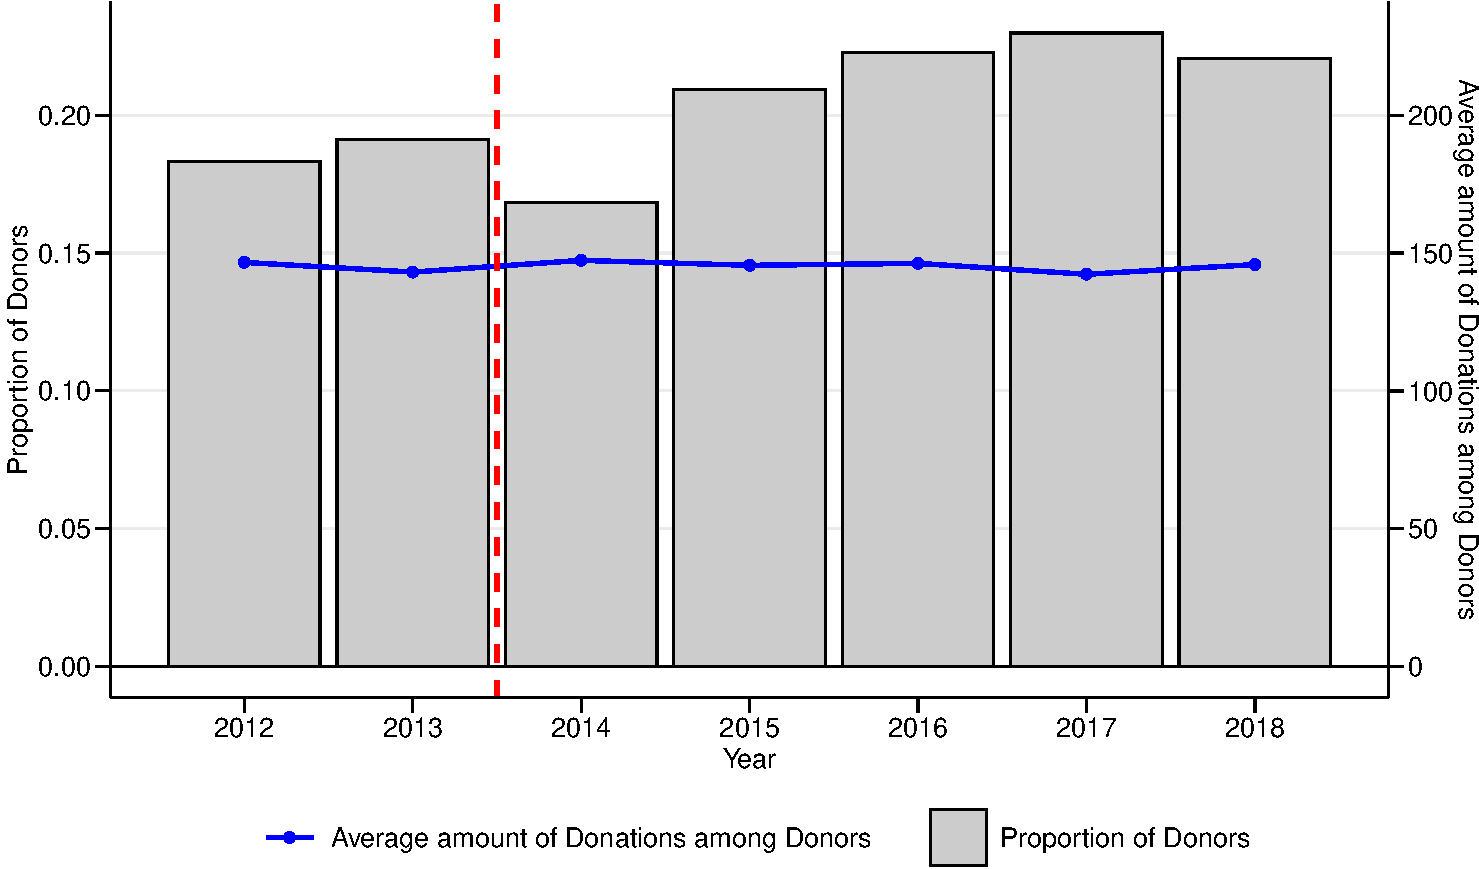
\includegraphics[width=0.7\linewidth,]{C:/Users/katoo/Desktop/NASTAB/paper/slide_files/figure-beamer/SummaryOutcome-1} 

}

\caption{Proportion of Donors and Average Donations among Donors. Notes: The left and right axises measure prooortion of donors and the average amount of donations among donors, respectively. Authors made this graph based on NaSTaB data.}\label{fig:SummaryOutcome}
\end{figure}
\end{frame}

\begin{frame}{Distribution of Charitable Giving}
\protect\hypertarget{distribution-of-charitable-giving}{}
\begin{figure}[t]

{\centering 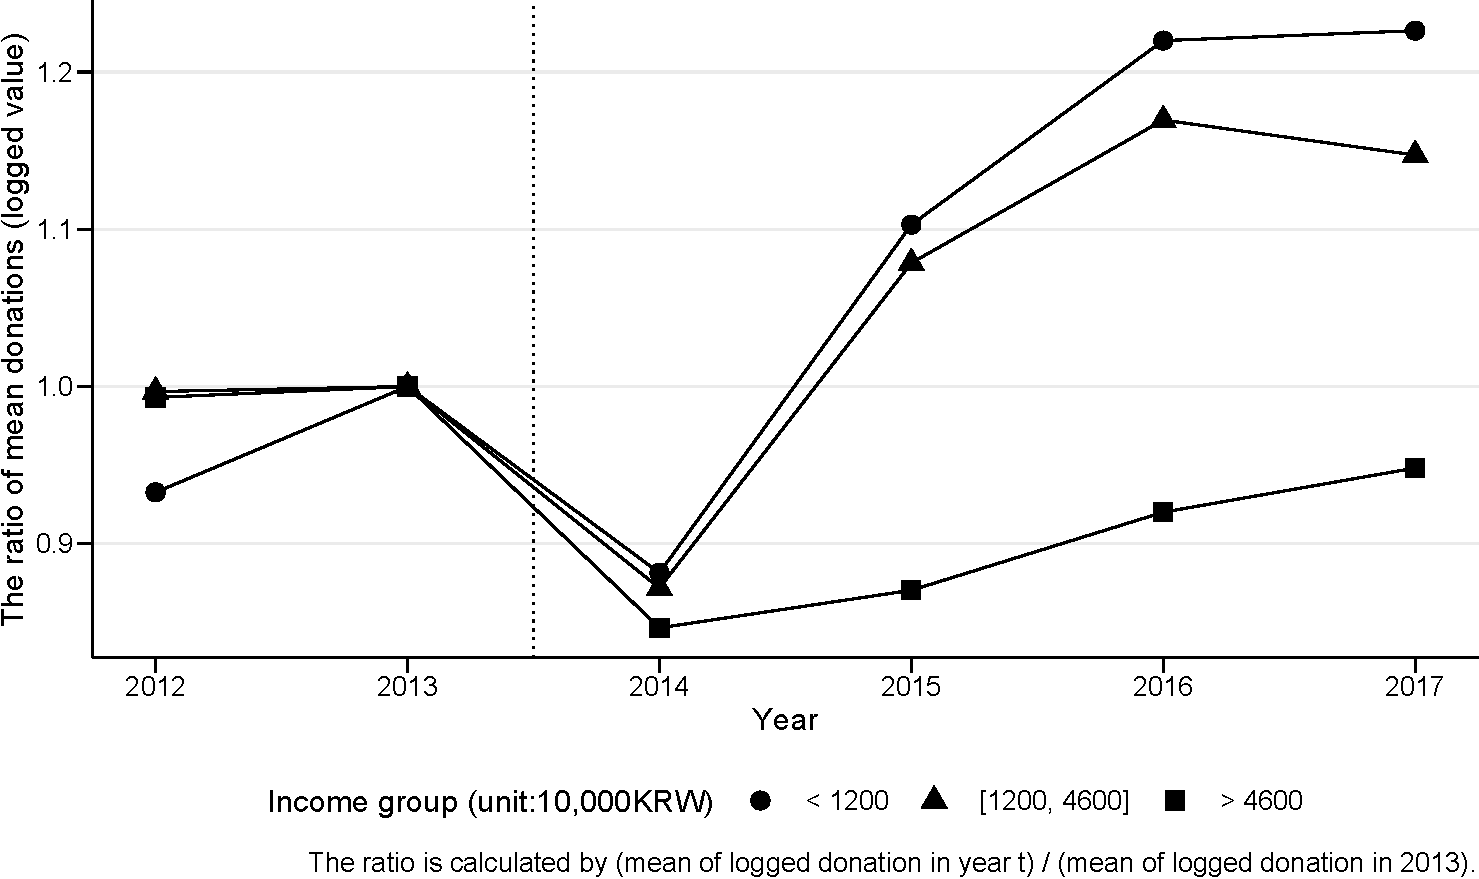
\includegraphics[width=0.85\linewidth,]{C:/Users/katoo/Desktop/NASTAB/paper/slide_files/figure-beamer/SummaryOutcome2-1} 

}

\caption{Distribution of Charitable Giving among Those Who Donated}\label{fig:SummaryOutcome2}
\end{figure}
\end{frame}

\begin{frame}{Proportion of Donors By Having Applied for Tax Relief}
\protect\hypertarget{proportion-of-donors-by-having-applied-for-tax-relief}{}
\begin{figure}[t]

{\centering 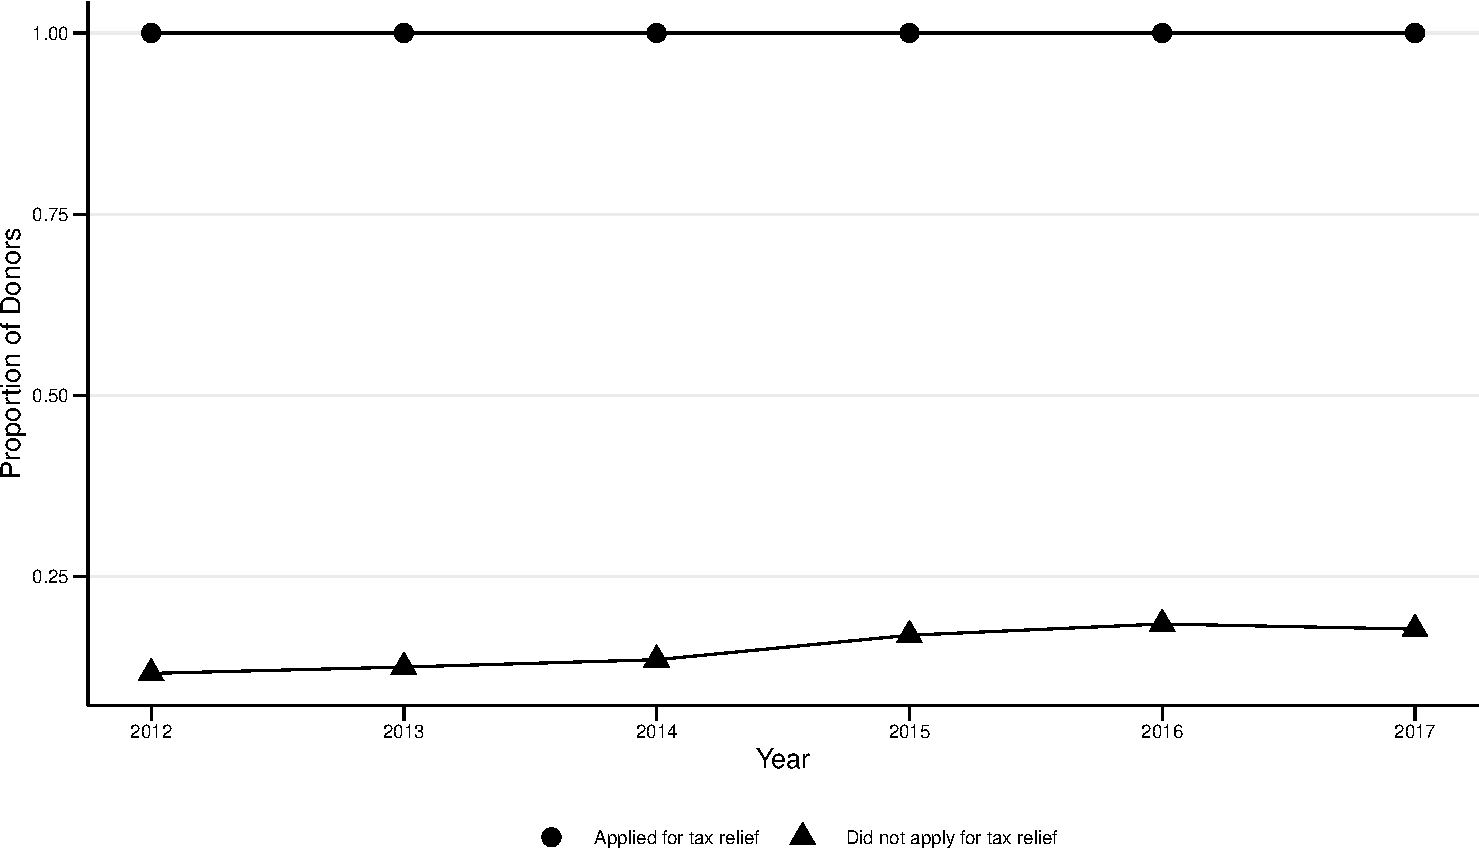
\includegraphics[width=0.85\linewidth,]{C:/Users/katoo/Desktop/NASTAB/paper/slide_files/figure-beamer/SummaryOutcome3-1} 

}

\caption{Proportion of Donors By Having Applied for Tax Relief}\label{fig:SummaryOutcome3}
\end{figure}
\end{frame}

\begin{frame}{Income Distribution and Giving Price}
\protect\hypertarget{income-distribution-and-giving-price}{}
\begin{figure}[t]

{\centering 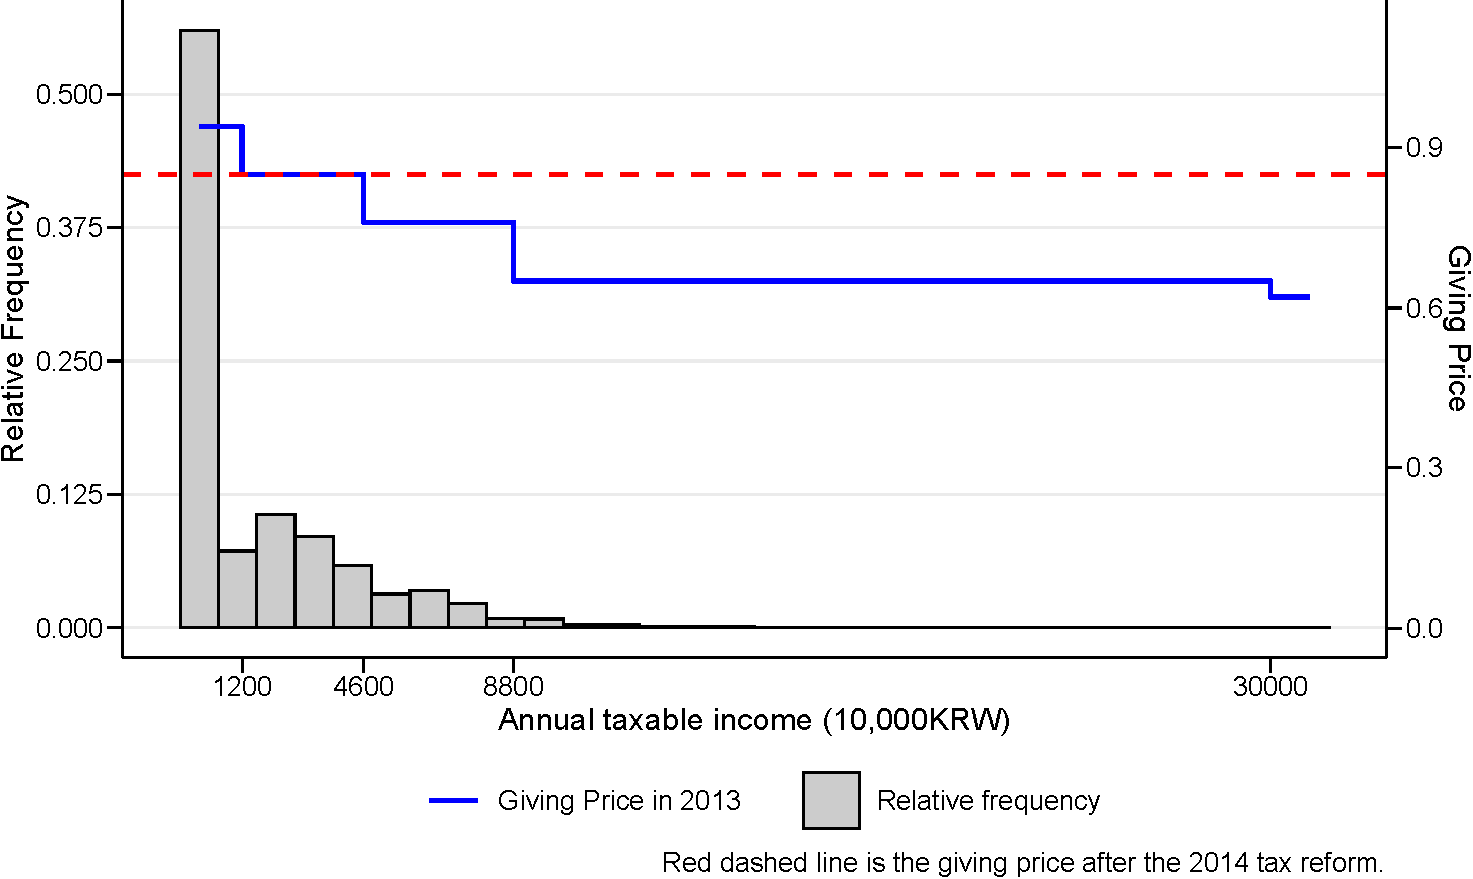
\includegraphics[width=0.7\linewidth,]{C:/Users/katoo/Desktop/NASTAB/paper/slide_files/figure-beamer/SummaryPrice-1} 

}

\caption{Income Distribution and Relative Giving Price in 2013. Notes: The left and right axis measure the relative frequency of respondents and the relative giving price, respectively. A blue step line and a red dashed horizontal line represents the giving price in 2013 and 2014, respectively. The grey bar shows income distribution in 2013.}\label{fig:SummaryPrice}
\end{figure}
\end{frame}

\begin{frame}{Charitable Giving by Income Group (Overall)}
\protect\hypertarget{charitable-giving-by-income-group-overall}{}
\begin{figure}[t]

{\centering 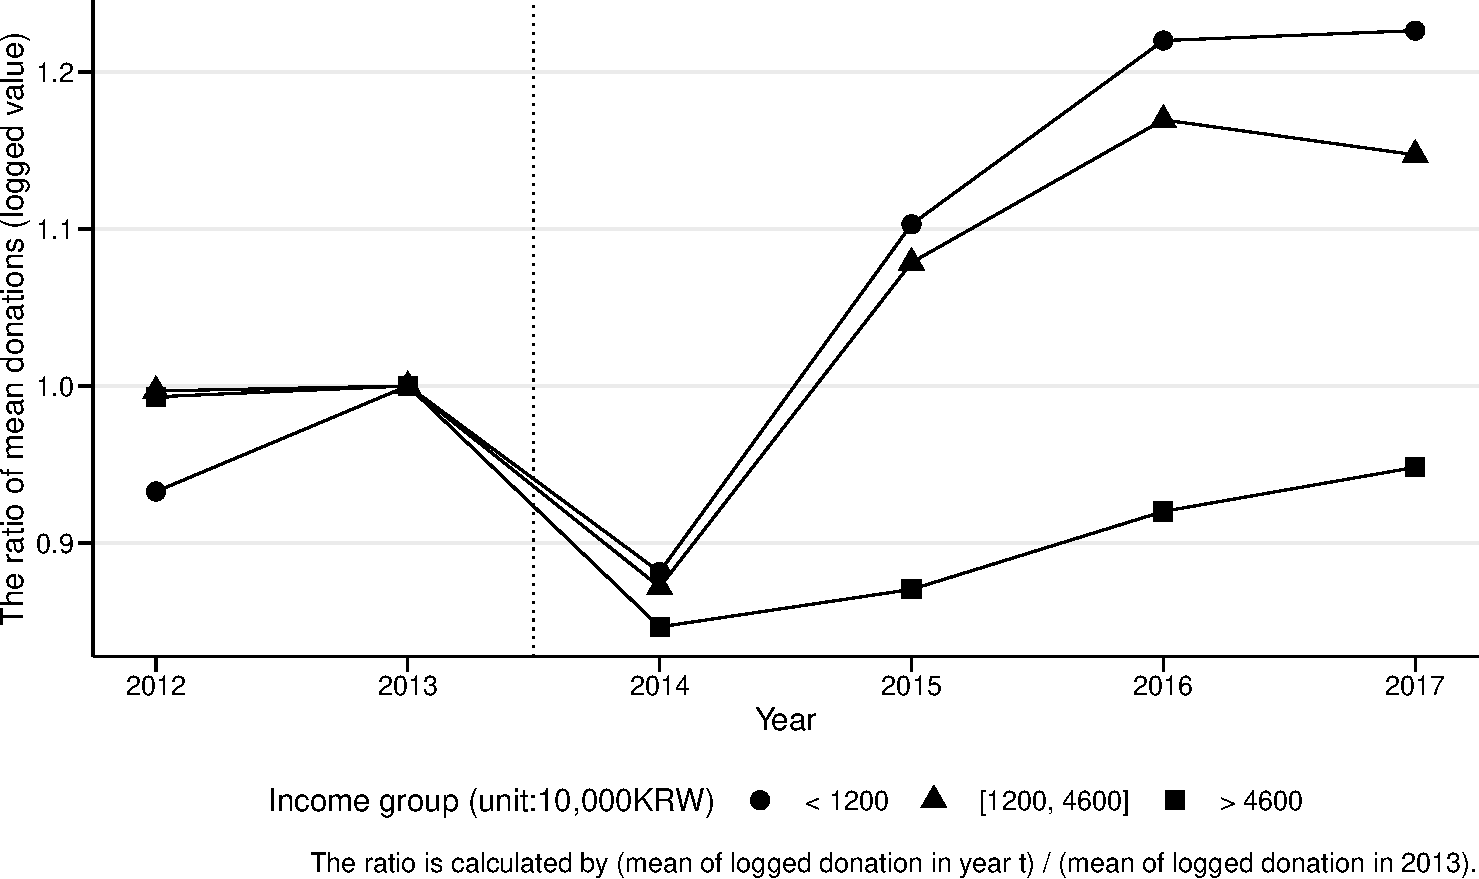
\includegraphics[width=0.7\linewidth,]{C:/Users/katoo/Desktop/NASTAB/paper/slide_files/figure-beamer/SummaryOutcome4-1} 

}

\caption{Average Logged Giving in Three Income Groups. Notes: We created three income groups, with the relative price of giving rising (circle), unchanged (triangle), and falling (square) between 2013 and 2014.}\label{fig:SummaryOutcome4}
\end{figure}
\end{frame}

\begin{frame}{Charitable Giving by Income Group (Intensive Margin)}
\protect\hypertarget{charitable-giving-by-income-group-intensive-margin}{}
\begin{figure}[t]

{\centering 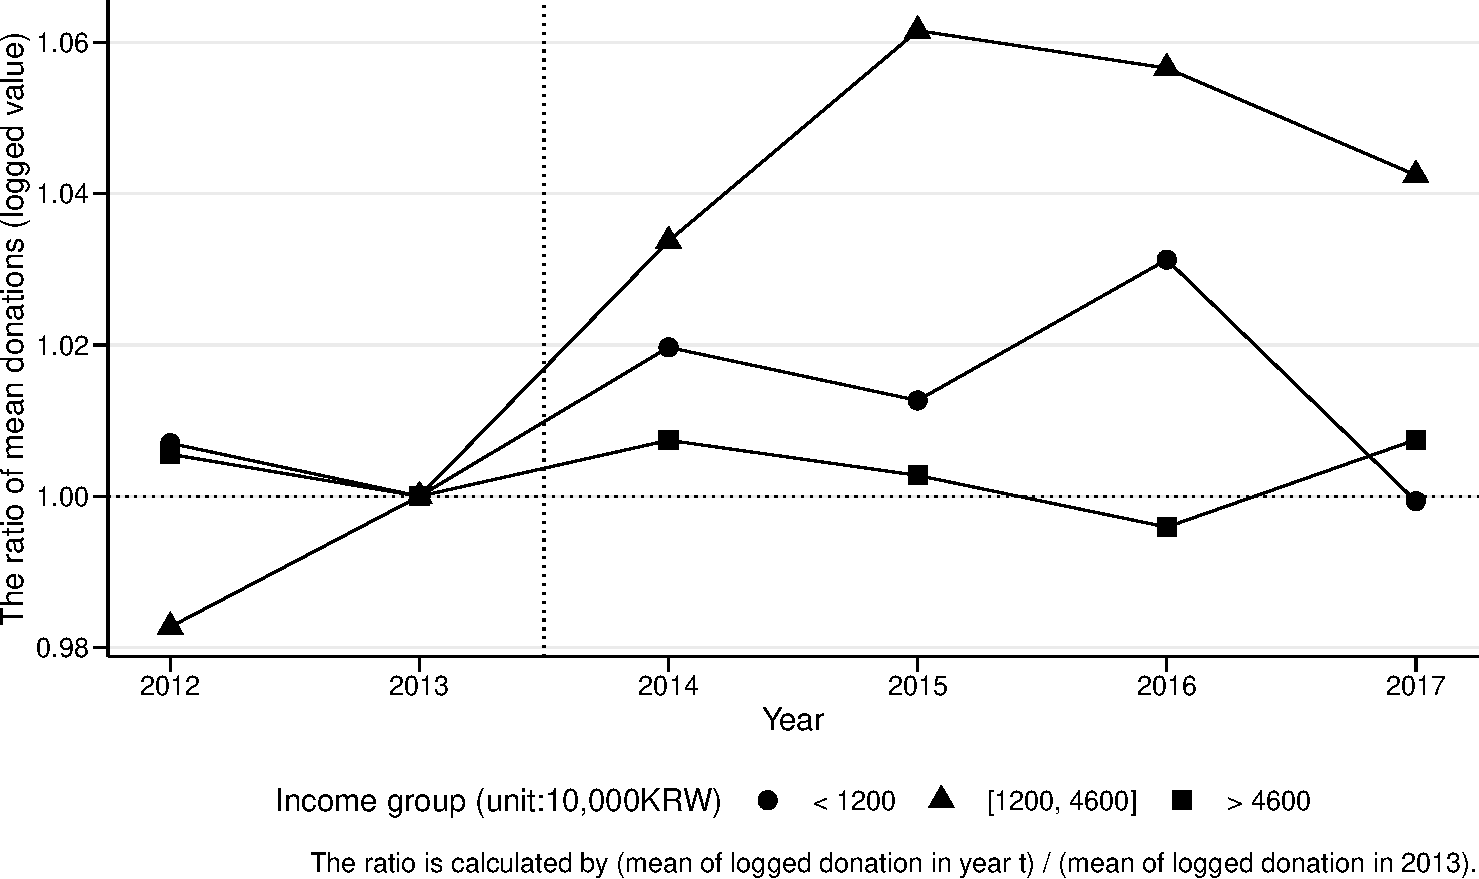
\includegraphics[width=0.7\linewidth,]{C:/Users/katoo/Desktop/NASTAB/paper/slide_files/figure-beamer/SummaryOutcome5-1} 

}

\caption{Average Logged Giving in Three Income Groups. Notes: We created three income groups, with the relative price of giving rising (circle), unchanged (triangle), and falling (square) between 2013 and 2014.}\label{fig:SummaryOutcome5}
\end{figure}
\end{frame}

\begin{frame}{Charitable Giving by Income Group (Extensive Margin)}
\protect\hypertarget{charitable-giving-by-income-group-extensive-margin}{}
\begin{figure}[t]

{\centering 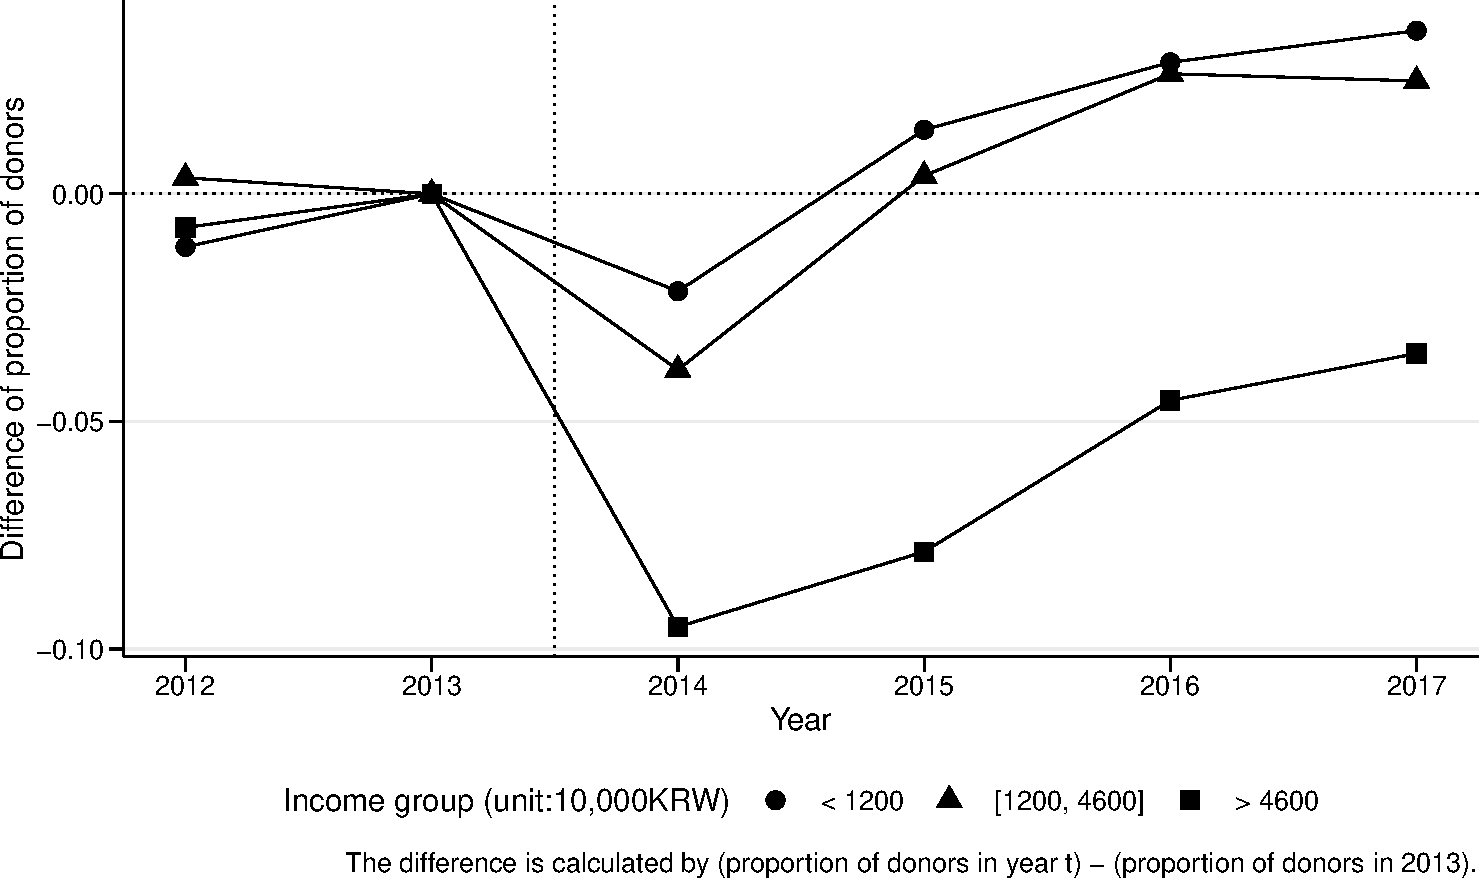
\includegraphics[width=0.7\linewidth,]{C:/Users/katoo/Desktop/NASTAB/paper/slide_files/figure-beamer/SummaryOutcome6-1} 

}

\caption{Proportion of Donors in Three Income Groups. Notes: We created three income groups, with the relative price of giving rising (circle), unchanged (triangle), and falling (square) between 2013 and 2014.}\label{fig:SummaryOutcome6}
\end{figure}
\end{frame}

\begin{frame}{Share of Tax Relief Grouped by Wage Earner or not}
\protect\hypertarget{share-of-tax-relief-grouped-by-wage-earner-or-not}{}
\begin{figure}[t]

{\centering 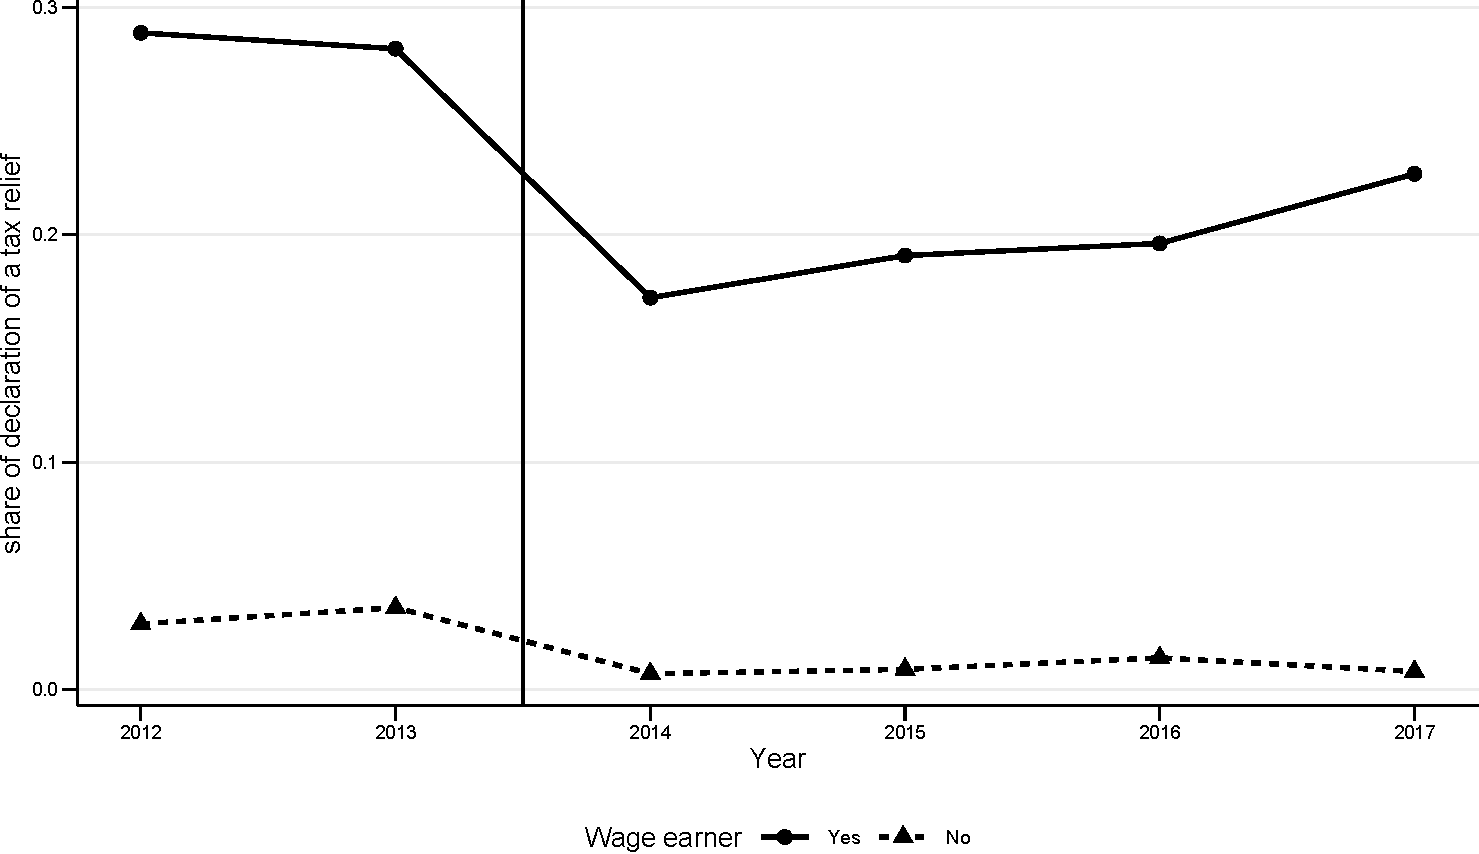
\includegraphics[width=0.7\linewidth,]{C:/Users/katoo/Desktop/NASTAB/paper/slide_files/figure-beamer/SummaryRelief-1} 

}

\caption{Share of Tax Relief. Notes: A solid line is the share of applying for tax relief among wage eaners. A dashed line is the share of applying for tax relief other than wage earners.}\label{fig:SummaryRelief}
\end{figure}
\end{frame}

\begin{frame}{Share of Tax Relief Grouped By Three Income Group}
\protect\hypertarget{share-of-tax-relief-grouped-by-three-income-group}{}
\begin{figure}[t]

{\centering 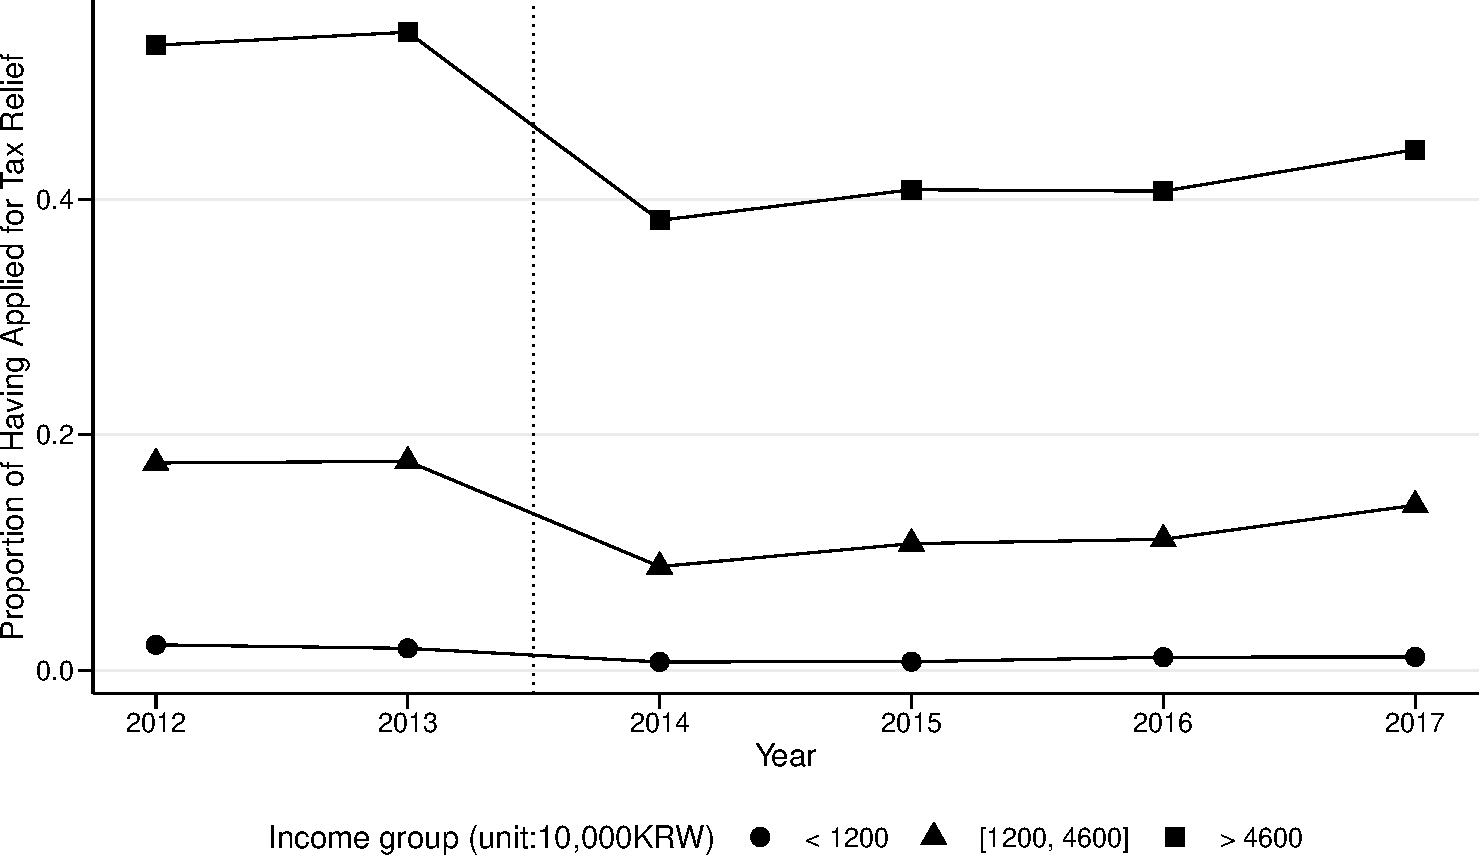
\includegraphics[width=0.85\linewidth,]{C:/Users/katoo/Desktop/NASTAB/paper/slide_files/figure-beamer/SummaryRelief2-1} 

}

\caption{Proportion of Having Applied for Tax Relief in Three Income Groups. Notes: We created three income groups, with the relative price of giving rising (circle), unchanged (triangle), and falling (square) between 2013 and 2014.}\label{fig:SummaryRelief2}
\end{figure}
\end{frame}

\hypertarget{first-stage-result-who-applied-for-tax-relief}{%
\section{First-Stage Result: Who Applied for Tax Relief?}\label{first-stage-result-who-applied-for-tax-relief}}

\begin{frame}{Probit Estimation of Selection of Applying for Tax Relief}
\protect\hypertarget{probit-estimation-of-selection-of-applying-for-tax-relief}{}
\begin{table}
\centering
\fontsize{6}{8}\selectfont
\begin{threeparttable}
\begin{tabular}[t]{lccccccc}
\toprule
\multicolumn{2}{c}{ } & \multicolumn{6}{c}{Separated Probit Model} \\
\cmidrule(l{3pt}r{3pt}){3-8}
  & Pooled & 2012 & 2013 & 2014 & 2015 & 2016 & 2017\\
\midrule
Wage earner & 0.478*** & 0.457*** & 0.228** & 0.611*** & 0.538*** & 0.440*** & 0.809***\\
 & (0.069) & (0.097) & (0.095) & (0.133) & (0.122) & (0.107) & (0.130)\\
\# Tax accountant & 0.852** & 0.110 & -0.464 & -0.204 & -0.178 & -0.293 & -0.130\\
 & (0.363) & (0.584) & (0.442) & (0.373) & (0.241) & (0.221) & (0.244)\\
log(first price) & -0.150 & -1.132 & -1.979** &  &  &  & \\
 & (0.271) & (0.884) & (0.873) &  &  &  & \\
log(income) & 18.959*** & 15.896*** & 16.033*** & 18.768*** & 19.124*** & 17.022*** & 21.084***\\
 & (1.025) & (3.049) & (2.993) & (1.514) & (1.399) & (1.334) & (1.354)\\
Age & 0.041*** & 0.057*** & 0.036* & 0.044 & 0.023 & 0.027 & 0.058***\\
 & (0.006) & (0.021) & (0.020) & (0.027) & (0.024) & (0.022) & (0.022)\\
Square of age & -0.044*** & -0.062*** & -0.036* & -0.049 & -0.031 & -0.027 & -0.060**\\
 & (0.006) & (0.024) & (0.022) & (0.031) & (0.027) & (0.025) & (0.024)\\
female & 0.111*** & 0.012 & 0.216*** & 0.153* & 0.068 & 0.029 & 0.181***\\
 & (0.037) & (0.068) & (0.066) & (0.080) & (0.075) & (0.072) & (0.069)\\
University graduate & 0.183*** & 0.294** & 0.262* & 0.150 & 0.194 & 0.268 & -0.098\\
 & (0.056) & (0.149) & (0.139) & (0.192) & (0.191) & (0.180) & (0.166)\\
Highschool graduate & 0.138*** & 0.265* & 0.224* & 0.044 & 0.171 & 0.172 & -0.092\\
 & (0.051) & (0.144) & (0.133) & (0.188) & (0.187) & (0.176) & (0.162)\\
\midrule
Num.Obs. & 26922 & 4261 & 4391 & 4383 & 4550 & 4611 & 4726\\
Log.Lik. & -7489.763 & -1383.811 & -1432.453 & -977.129 & -1116.751 & -1181.082 & -1267.813\\
Std. Errors & Clustered (year) & Standard & Standard & Standard & Standard & Standard & Standard\\
FE: year & X &  &  &  &  &  & \\
\bottomrule
\end{tabular}
\begin{tablenotes}
\item Notes: $^{*}$ $p < 0.1$, $^{**}$ $p < 0.05$, $^{***}$ $p < 0.01$.
\end{tablenotes}
\end{threeparttable}
\end{table}
\end{frame}

\hypertarget{estimating-conventional-price-elasticities}{%
\section{Estimating Conventional Price Elasticities}\label{estimating-conventional-price-elasticities}}

\begin{frame}{Intensive-Margin Price Elasticity}
\protect\hypertarget{intensive-margin-price-elasticity}{}
\begin{table}
\centering
\fontsize{7}{9}\selectfont
\begin{threeparttable}
\begin{tabular}[t]{lccccc}
\toprule
\multicolumn{1}{c}{ } & \multicolumn{3}{c}{FE} & \multicolumn{2}{c}{FE-2SLS} \\
\cmidrule(l{3pt}r{3pt}){2-4} \cmidrule(l{3pt}r{3pt}){5-6}
  & (1) & (2) & (3) & (4) & (5)\\
\midrule
Application x log(first price) & -0.851*** &  &  & -0.813 & -1.716*\\
 & (0.219) &  &  & (0.854) & (0.907)\\
PS of application x log(first price) &  & -1.527*** & -1.561*** &  & \\
 &  & (0.371) & (0.354) &  & \\
\midrule
Num.Obs. & 7109 & 7080 & 7080 & 7080 & 7080\\
R2 & 0.820 & 0.820 & 0.820 & 0.820 & 0.820\\
First-stage: Instrument &  &  &  & -0.360 & -0.250\\
 &  &  &  & [162.5] & [181.0]\\
R2 Adj. & 0.693 & 0.693 & 0.694 & 0.694 & 0.692\\
FE: area & X & X & X & X & X\\
FE: industry & X & X & X & X & X\\
FE: panelid & X & X & X & X & X\\
FE: year & X & X & X & X & X\\
Square of age & X & X & X & X & X\\
Method of Propensity Score &  & Pooled & Separated & Pooled & Separated\\
\bottomrule
\end{tabular}
\begin{tablenotes}
\item Notes: $^{*}$ $p < 0.1$, $^{**}$ $p < 0.05$, $^{***}$ $p < 0.01$. Standard errors are clustered at individual level. A square bracket is wald statistics of instrument.
\end{tablenotes}
\end{threeparttable}
\end{table}
\end{frame}

\begin{frame}{Extensive-Margin Price Elasticity}
\protect\hypertarget{extensive-margin-price-elasticity}{}
\begin{table}
\centering
\fontsize{7}{9}\selectfont
\begin{threeparttable}
\begin{tabular}[t]{lccccc}
\toprule
\multicolumn{1}{c}{ } & \multicolumn{3}{c}{FE} & \multicolumn{2}{c}{FE-2SLS} \\
\cmidrule(l{3pt}r{3pt}){2-4} \cmidrule(l{3pt}r{3pt}){5-6}
  & (1) & (2) & (3) & (4) & (5)\\
\midrule
Application x log(first price) & -2.759*** &  &  & -1.401*** & -1.847***\\
 & (0.074) &  &  & (0.208) & (0.193)\\
PS of application x log(first price) &  & -0.474*** & -0.563*** &  & \\
 &  & (0.103) & (0.097) &  & \\
\midrule
Num.Obs. & 27076 & 26922 & 26922 & 26922 & 26922\\
R2 & 0.717 & 0.663 & 0.663 & 0.704 & 0.712\\
First-stage: Instrument &  &  &  & -0.275 & -0.216\\
 &  &  &  & [347.9] & [375.7]\\
Implied price elasticity & -10.509*** & -1.804*** & -2.141*** & -5.326*** & -7.024***\\
 & (0.281) & (0.390) & (0.369) & (0.792) & (0.733)\\
R2 Adj. & 0.620 & 0.547 & 0.547 & 0.603 & 0.613\\
FE: area & X & X & X & X & X\\
FE: industry & X & X & X & X & X\\
FE: panelid & X & X & X & X & X\\
FE: year & X & X & X & X & X\\
Square of age & X & X & X & X & X\\
\bottomrule
\end{tabular}
\begin{tablenotes}
\item Notes: $^{*}$ $p < 0.1$, $^{**}$ $p < 0.05$, $^{***}$ $p < 0.01$. Standard errors are clustered at individual level. A square bracket is wald statistics of instrument.
\end{tablenotes}
\end{threeparttable}
\end{table}
\end{frame}

\hypertarget{control-function-approach}{%
\section{Control Function Approach}\label{control-function-approach}}

\begin{frame}{Estimation of Outcome Equation for \(R_{it} = 1\)}
\protect\hypertarget{estimation-of-outcome-equation-for-r_it-1}{}
\begin{table}
\centering
\fontsize{7}{9}\selectfont
\begin{threeparttable}
\begin{tabular}[t]{lccc}
\toprule
  & (1) & (2) & (3)\\
\midrule
log(first price) & -1.325*** & -1.307*** & -1.279***\\
 & (0.386) & (0.384) & (0.387)\\
log(income) & 2.030 & 1.455 & 3.957*\\
 & (1.515) & (1.837) & (2.229)\\
Selection correction term (separate) &  & -0.056 & \\
 &  & (0.133) & \\
Selection correction term (pool) &  &  & 0.209\\
 &  &  & (0.193)\\
\midrule
Num.Obs. & 3646 & 3643 & 3643\\
R2 & 0.839 & 0.839 & 0.839\\
R2 Adj. & 0.726 & 0.725 & 0.726\\
FE: area & X & X & X\\
FE: industry & X & X & X\\
FE: panelid & X & X & X\\
FE: year & X & X & X\\
Square of Age & X & X & X\\
\bottomrule
\end{tabular}
\begin{tablenotes}
\item Notes: $^{*}$ $p < 0.1$, $^{**}$ $p < 0.05$, $^{***}$ $p < 0.01$.
\end{tablenotes}
\end{threeparttable}
\end{table}
\end{frame}

\begin{frame}{Estimation of Outcome Equation for \(R_{it} = 0\)}
\protect\hypertarget{estimation-of-outcome-equation-for-r_it-0}{}
\begin{table}
\centering
\fontsize{7}{9}\selectfont
\begin{threeparttable}
\begin{tabular}[t]{lcccccc}
\toprule
\multicolumn{1}{c}{ } & \multicolumn{3}{c}{Intensive} & \multicolumn{3}{c}{Extensive} \\
\cmidrule(l{3pt}r{3pt}){2-4} \cmidrule(l{3pt}r{3pt}){5-7}
  & (1) & (2) & (3) & (4) & (5) & (6)\\
\midrule
log(income) & 0.696 & 2.765 & 4.660 & 0.535** & 0.513 & 0.524\\
 & (1.613) & (3.186) & (4.188) & (0.249) & (0.352) & (0.405)\\
Selection correction term (separate) &  & -0.176 &  &  & 0.001 & \\
 &  & (0.248) &  &  & (0.031) & \\
Selection correction term (pool) &  &  & -0.340 &  &  & 0.000\\
 &  &  & (0.305) &  &  & (0.040)\\
\midrule
Num.Obs. & 3463 & 3437 & 3437 & 23430 & 23279 & 23279\\
R2 & 0.865 & 0.866 & 0.866 & 0.580 & 0.580 & 0.580\\
R2 Adj. & 0.685 & 0.687 & 0.687 & 0.419 & 0.420 & 0.420\\
FE: area & X & X & X & X & X & X\\
FE: industry & X & X & X & X & X & X\\
FE: panelid & X & X & X & X & X & X\\
FE: year & X & X & X & X & X & X\\
Square of Age & X & X & X & X & X & X\\
\bottomrule
\end{tabular}
\begin{tablenotes}
\item Notes: $^{*}$ $p < 0.1$, $^{**}$ $p < 0.05$, $^{***}$ $p < 0.01$.
\end{tablenotes}
\end{threeparttable}
\end{table}
\end{frame}

\begin{frame}{Estimating Effect of Tax Incentive}
\protect\hypertarget{estimating-effect-of-tax-incentive}{}
\begin{table}
\centering
\begin{tabular}[t]{llrrr}
\toprule
Outcome & Include correction term? & ATE & ATT & ATU\\
\midrule
extensive & No & 0.834 & 0.624 & 0.852\\
 & Pool & 0.834 & 0.623 & 0.852\\
 & Separate & 0.834 & 0.622 & 0.852\\
intensive & No & 0.112 & 0.151 & 0.086\\
 & Pool & 0.062 & 0.416 & -0.178\\
 & Separate & 0.206 & 0.283 & 0.153\\
\bottomrule
\end{tabular}
\end{table}
\end{frame}

\hypertarget{welfare-implication}{%
\section{Welfare Implication}\label{welfare-implication}}

\begin{frame}{Partial Effect of Price (Subsets with \(R_{it} = 0\))}
\protect\hypertarget{partial-effect-of-price-subsets-with-r_it-0}{}
\begin{table}
\centering
\fontsize{7}{9}\selectfont
\begin{threeparttable}
\begin{tabular}[t]{lccc}
\toprule
  & (1) & (2) & (3)\\
\midrule
First price & 46.257 & 77.970 & 56.066\\
 & (147.244) & (156.865) & (147.440)\\
log(income) & -256.907 & -965.220 & -646.690\\
 & (425.966) & (1025.181) & (807.601)\\
Correction term &  & 69.254 & 42.673\\
 &  & (70.117) & (56.301)\\
\midrule
Num.Obs. & 3463 & 3437 & 3437\\
R2 Adj. & 0.622 & 0.622 & 0.622\\
FE: area & X & X & X\\
FE: industry & X & X & X\\
FE: panelid & X & X & X\\
FE: year & X & X & X\\
Square age & X & X & X\\
Method of IMR &  & Pooled & Separate\\
\bottomrule
\end{tabular}
\begin{tablenotes}
\item Notes: $^{*}$ $p < 0.1$, $^{**}$ $p < 0.05$, $^{***}$ $p < 0.01$. Standard errors are clustered at individual level.
\end{tablenotes}
\end{threeparttable}
\end{table}
\end{frame}

\begin{frame}{Improve Welfare by Increasing Tax Incentive}
\protect\hypertarget{improve-welfare-by-increasing-tax-incentive}{}
\begin{table}
\centering
\fontsize{6}{8}\selectfont
\begin{threeparttable}
\begin{tabular}[t]{lrrrr}
\toprule
model & Elasticity (R = 1) & Partial Effect (R = 0) & Sum of Giving (R = 1) & Partial Effect (R = 0) / Sum of Giving (R = 1)\\
\midrule
(1) & 1.325 & 160187.730 & 639992.100 & 0.250\\
(2) & 1.307 & 267982.430 & 639992.100 & 0.419\\
(3) & 1.279 & 192700.418 & 639992.100 & 0.301\\
\bottomrule
\end{tabular}
\begin{tablenotes}
\item Partial effect for R = 0 is multiplied by observations.
\end{tablenotes}
\end{threeparttable}
\end{table}
\end{frame}

\hypertarget{conclusion}{%
\section{Conclusion}\label{conclusion}}

\hypertarget{references}{%
\section*{References}\label{references}}
\addcontentsline{toc}{section}{References}

\begin{frame}{References}
\hypertarget{refs}{}
\begin{CSLReferences}{1}{0}
\leavevmode\vadjust pre{\hypertarget{ref-Almunia2020}{}}%
Almunia, M., Guceri, I., Lockwood, B., Scharf, K., 2020. More giving or more givers? The effects of tax incentives on charitable donations in the UK. Journal of Public Economics 183. doi:\href{https://doi.org/10.1016/j.jpubeco.2019.104114}{10.1016/j.jpubeco.2019.104114}

\leavevmode\vadjust pre{\hypertarget{ref-Auten2002}{}}%
Auten, G.E., Sieg, H., Clotfelter, C.T., 2002. \href{http://www.jstor.org/stable/3083340}{Charitable giving, income, and taxes: An analysis of panel data}. American Economic Review 92, 371--382.

\leavevmode\vadjust pre{\hypertarget{ref-Fack2016}{}}%
Fack, G., Landais, C., 2016. The effect of tax enforcement on tax elasticities: Evidence from charitable contributions in france. Journal of Public Economics 133, 23--40. doi:\url{https://doi.org/10.1016/j.jpubeco.2015.10.004}

\leavevmode\vadjust pre{\hypertarget{ref-Gillitzer2018}{}}%
Gillitzer, C., Skov, P.E., 2018. {The use of third-party information reporting for tax deductions: evidence and implications from charitable deductions in Denmark}. Oxford Economic Papers 70, 892--916. doi:\href{https://doi.org/10.1093/oep/gpx055}{10.1093/oep/gpx055}

\leavevmode\vadjust pre{\hypertarget{ref-Saez2004}{}}%
Saez, E., 2004. The optimal treatment of tax expenditures. Journal of Public Economics 88, 2657--2684. doi:\href{https://doi.org/10.1016/j.jpubeco.2003.09.004}{10.1016/j.jpubeco.2003.09.004}

\end{CSLReferences}
\end{frame}

\end{document}
